\documentclass{article}
\usepackage[utf8]{inputenc}
\usepackage[left=1cm,right=0.5cm,bottom=0.5cm,top=0.5cm]{geometry}
\usepackage{setspace}
\usepackage{graphicx}
\usepackage{amsmath}
\usepackage{graphbox}
\usepackage{enumitem}
\setstretch{0.8}
\setlist{nosep}

% 1 side of paper
\begin{document}
\begin{center}
    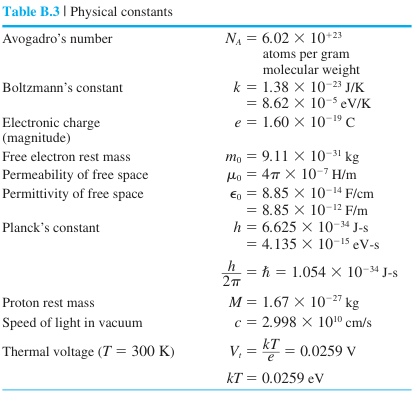
\includegraphics[align=c, width=9cm]{consts.png}
    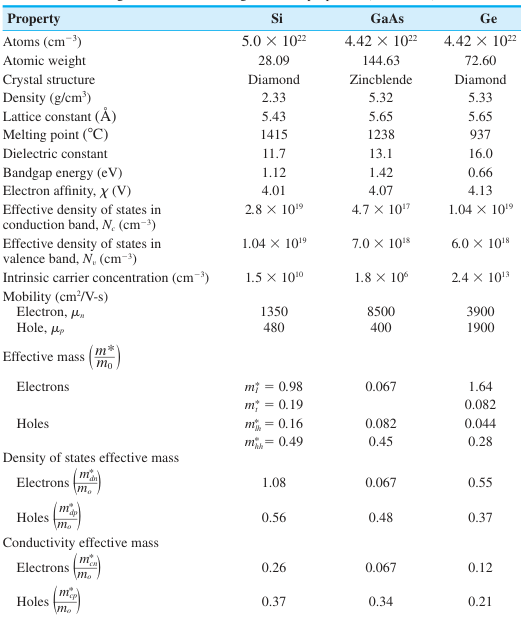
\includegraphics[align=c, width=9cm]{props.png}
\end{center}
% TODO: Chapter 1 concepts? Not many formulas up here, mostly concepts and geometry
\textbf{Basics of solids}
\begin{itemize}
    \item $E_c$ is the min energy of the conduction band, $E_v$ is the max energy of the valence band, $E_g$ is the bandgap ($E_c - E_v$)
    \item Density of states
    \begin{itemize}
        \item Conduction band: $g_c(E) = \frac{4 \pi (2m_n^*)^{3/2}}{h^3} \sqrt{E - E_c}$, Valence band: $g_v(E) = \frac{4 \pi (2m_p^*)^{3/2}}{h^3} \sqrt{E_v - E}$
    \end{itemize}
    \item Fermi-Dirac probability
    \begin{itemize}
        \item Probable distribution function: $f_F(E) = \frac{1}{1 + exp\left(\frac{E - E_F}{kT}\right)}$
        \item $f_F(E_F) = \frac{1}{2}$, and $E_F$ is known as the Fermi energy. Kind of the "center" of the distribution
        \item Boltzmann approx (when $E - E_F >> kT$): $f_F(E) \approx exp\left[\frac{-(E - E_F)}{kT}\right]$
    \end{itemize}
\end{itemize}
\textbf{Dopants}
\begin{itemize}
    \item Intrinsic semiconductor means no dopants at all, extrinsic semiconductor means doped
    \item When $n_0 > p_0$, semiconductor is N-type (majority donors), and when $p_0 > n_0$, semiconductor is P-type (majority acceptors)
    \item Thermal equilibrium carrier concentrations
    \begin{itemize}
        \item Electron concentration (unit is $cm^{-3}$): $n_0 = N_c \cdot exp\left[\frac{-(E_c - E_F)}{kT}\right]$, $n_0 \propto N_c$
        \item Hole concentration (unit is $cm^{-3}$): $p_0 = N_v \cdot exp\left[\frac{-(E_F - E_v)}{kT}\right]$, $p_0 \propto N_v$
        \item $N_c$ and $N_v$ are the "effective density of states", and are \textbf{very temperature dependent} with $N = N_{T0} \cdot \frac{T}{T_0}^{3/2}$.
        \item For an intrinsic semiconductor, $n_i = p_i$, and $n_i^2 = N_c N_v exp\left[\frac{-E_g}{kT}\right]$
        \item For intrinsic AND extrinsic semiconductors, $n_0 \cdot p_0 = n_i^2$
    \end{itemize}
    \item Donor Fermi-Dirac probability
    \begin{itemize}
        \item $n_d = \frac{N_d}{1 + \frac{1}{2}exp\left(\frac{E_d - E_F}{kT}\right)}$
        \item $p_a = \frac{N_a}{1 + \frac{1}{g}exp\left(\frac{E_F - E_a}{kT}\right)}$, $g$ is a "degeneracy factor" that's 4 for Si and GaAs.
    \end{itemize}
    \item Compenated semiconductors
    \begin{itemize}
        \item $n_0 = \frac{N_d - N_a}{2} + \sqrt{\left(\frac{N_d - N_a}{2}\right)^2 + n_i^2}$, $p_0 = \frac{N_a - N_d}{2} + \sqrt{\left(\frac{N_a - N_d}{2}\right)^2 + n_i^2}$
    \end{itemize}
    % TODO: This is also 4.5 so read up before finishing
    \item Fermi energy modelling
    \begin{itemize}
        \item For an intrinsic semiconductor, $E_{Fi} - E_{midgap} = \frac{3}{4} kT \ln \left(\frac{m_p^*}{m_n^*}\right)$
    \end{itemize}
\end{itemize}
\end{document}
